\documentclass{ximera}

\newcommand{\RR}{\mathbb R}
\renewcommand{\d}{\,d}
\newcommand{\dd}[2][]{\frac{d #1}{d #2}}
\renewcommand{\l}{\ell}
\newcommand{\ddx}{\frac{d}{dx}}
\newcommand{\dfn}{\textbf}
\newcommand{\eval}[1]{\bigg[ #1 \bigg]}


\outcome{Understand the connection between curves and parameterizations.}

\author{Jim Talamo}

\begin{document}
\begin{exercise}
 A portion of the curve $\mathcal{C}$ traced out by  $\vec{p}(t)$ is shown below.  The points associated to $\vec{p}(t)$ for various $t$values are shown on the curve.

\begin{center}
\resizebox {5cm} {!} { 
    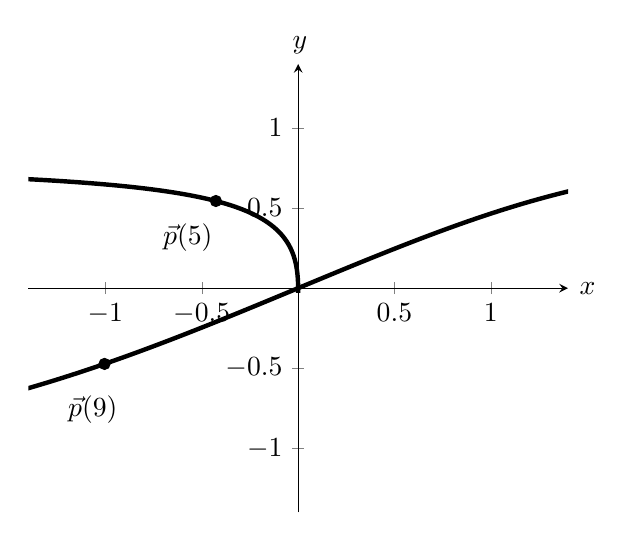
\begin{tikzpicture}
      \begin{axis}[
          xmin=-1.4, xmax=1.4, ymin =-1.4, ymax = 1.4,
          axis lines=center,  
          xlabel=$x$,  
          ylabel=$y$,  
          every axis y label/.style={at=(current axis.above origin),anchor=south},  
          every axis x label/.style={at=(current axis.right of origin),anchor=west}
        ]
        \addplot [black,ultra thick,domain=0:90,smooth,samples=100] ({-((x/180)^(.3))*tan(x)+((x/180)^(.3))*sin(x)},{((x/180)^(.3))*sin(x)-.03});
        \addplot [black,ultra thick,domain=91:220,smooth,samples=100] ({-((x/180)^(.3))*tan(x)+((x/180)^(.3))*sin(x)},{((x/180)^(.3))*sin(x)});
%        \node[above right,black] at (axis cs: 0,-.3) {$\vec{p}(0)$};
%        \node[above right,black] at (axis cs: -1.3,0) {$\vec{p}(4)$};
        \node[above right,black] at (axis cs: {-((110/180)^(.3))*tan(110)+((110/180)^(.3))*sin(110)},{((110/180)^(.3))*sin(110)}) {$\vec{p}(2)$};
        \node[above left,black] at (axis cs: {-((45/180)^(.3))*tan(45)-.1+((45/180)^(.3))*sin(45)-.1},{((45/180)^(.3))*sin(45)-.3}) {$\vec{p}(5)$};
        \node[above right,black] at (axis cs: {-((215/180)^(.3))*tan(215)+.1+((215/180)^(.3))*sin(215)},{((215/180)^(.3))*sin(215)-.3}) {$\vec{p}(9)$};
        
        \addplot[color=black,fill=black,only marks,mark=*] coordinates{(-{((55/180)^(.3))*tan(55)+((55/180)^(.3))*sin(55)},{((55/180)^(.3))*sin(55)-.03})};
        \addplot[color=black,fill=black,only marks,mark=*] coordinates{(-{((110/180)^(.3))*tan(110)+((110/180)^(.3))*sin(110)},{((110/180)^(.3))*sin(110)})};
        \addplot[color=black,fill=black,only marks,mark=*] coordinates{(-{((207/180)^(.3))*tan(207)+((207/180)^(.3))*sin(207)},{((207/180)^(.3))*sin(207)})};
%        \addplot[color=black,fill=black,only marks,mark=*] coordinates{(-{((270/180)^(.3))*tan(270)+((270/180)^(.3))*sin(270)},{((270/180)^(.3))*sin(270)})};

        
      \end{axis}
    \end{tikzpicture}}
\end{center}

Provide the most accurate response to the following questions.  
 
 Which of the following vectors is orthogonal to $\vec{p}(5)?$
 \begin{multipleChoice}
 \choice{$\vector{1,0}$}
 \choice{$\vector{0,1}$}
 \choice[correct]{$\vector{1,1}$}
 \choice{$\vector{-1,1}$}
 \end{multipleChoice}
 
 Which of the following vectors is parallel to $\vec{p}'(5)?$
 \begin{multipleChoice}
 \choice{$\vector{1,0}$}
 \choice{$\vector{0,1}$}
 \choice{$\vector{-1,1}$}
 \choice{$\vector{1,5}$}
 \choice{$\vector{1,-5}$}
 \choice{$\vector{5,1}$}
 \choice[correct]{$\vector{5,-1}$}
 \end{multipleChoice}
 
 Which of the following vectors is parallel to $\vec{p}'(9)?$
 \begin{multipleChoice}
 \choice{$\vector{1,0}$}
 \choice{$\vector{0,1}$}
 \choice{$\vector{-1,1}$}
 \choice[correct]{$\vector{1,2}$}
 \choice{$\vector{1,-2}$}
 \choice{$\vector{2,1}$}
 \choice{$\vector{-2,1}$}
 \end{multipleChoice}
 
Which of the following vectors is parallel to $\vector{-x(9),y(5)}?$
 \begin{multipleChoice}
 \choice{$\vector{1,1}$}
 \choice{$\vector{1,-1}$}
 \choice{$\vector{1,2}$}
 \choice{$\vector{1,-2}$}
 \choice[correct]{$\vector{2,1}$}
 \choice{$\vector{2,-1}$}
 \choice{more than one of these.}
 \end{multipleChoice}
 
 \end{exercise}
\end{document}
